\documentclass[conference]{IEEEtran}
\usepackage[utf8]{inputenc}
\usepackage{booktabs}
\usepackage{caption}
\usepackage[portuguese]{babel}
\usepackage{graphicx}

\captionsetup[table]{labelformat=default, labelsep=period, textfont=bf}
\title{Comparação de Algoritmos de Categorização \\ \large Categorizar um veículo a partir das suas informações \\
\textit{Comparation of Categorization Algorithms \\ \large Categorize a vehicle based on its information}}
\author{
\IEEEauthorblockN{Martinho Caeiro - 23917 || Paulo Abade - 23919}
\IEEEauthorblockA{
    Instituto Politécnico de Beja\\
    Escola Superior de Tecnologia e Gestão\\
    Beja, Portugal\\
    23917@stu.ipbeja.pt || 23919@stu.ipbeja.pt
}
}

\begin{document}
\maketitle
\begin{figure}[!ht]
	\centering
	
\includegraphics[width=0.4\textwidth]{Resources/Logo/IPBejaESTIG.jpg}
\end{figure}

%----------------------------------------------------------------------------------------------------------------------------------------------
\begin{abstract}
	Este artigo apresenta um estudo para a comparação entre algoritmos de categorização de veículos. O objetivo de cada um dos
	algoritmos é categorizar um veículo a partir das suas informações, sendo que este veículo será categorizado consoante o seu
	país de origem. Foi escolhido este tema para facilitar a nossa compreensão sobre o assunto e tornar mais agradável o estudo
	destes algoritmos. O estudo foi realizado com base em algoritmos de aprendizagem supervisionada, nomeadamente o algoritmo
	\textit{Binary Tree}, algoritmo \textit{Random Forest} TODO: Escolher mais algoritmos para fazer a comparação entre eles.
	Para fazer a comparação destes, foi utilizado um dataset, com cerca de 400 entradas, onde possui informações de veículos de
	diferentes países e este foi utilizado nos diferentes algoritmos para treinar e testar os mesmos. Este dataset, já foi alterado
	no primeiro trabalho da Disciplina de \textit{Sistemas de Informação}, sendo ligeiramente diferente, por já ter sido tratado.
	Os resultados obtidos foram comparados e analisados para perceber qual o algoritmo que melhor categoriza um veículo a partir das
	suas informações. A comparação dos algoritmos foi feita com base na sua precisão, sensibilidade e especificidade. O estudo também
	abordou as limitações de cada algoritmo. Aplicações práticas incluem sistemas de recomendação de veículos, análise de dados ou apoio
	à criação de estratégias de marketing em diferentes regiões. A análise detalhada do comportamento dos algoritmos pode ser útil
	para investigadores e profissionais que desejam otimizar a categorização de grandes volumes de dados automóveis.

\end{abstract}

\begin{IEEEkeywords}
	algoritmos; veículos; categorização; aprendizagem supervisionada; árvore binária; random forest; precisão; sensibilidade; especificidade;
	orange; datamining; machine learning; kaggle.
\end{IEEEkeywords}

%----------------------------------------------------------------------------------------------------------------------------------------------
\section{Introdução}
A categorização de veículos é uma área relevante em aplicações práticas, como a otimização de cadeias de fornecimento, a personalização
de ofertas comerciais ou o desenvolvimento de sistemas inteligentes de transporte. Estudos recentes demonstram que algoritmos de
aprendizagem supervisionada podem oferecer soluções rápidas e eficazes para problemas de classificação, mas a escolha do algoritmo
adequado depende de vários fatores, como o tipo de dados e o objetivo final. Este estudo procura preencher essa lacuna, analisando não
apenas a precisão dos modelos, mas também os seus comportamentos sob diferentes métricas de avaliação. Para isso, foi utilizado um
dataset com informações de veículos de diferentes países, onde o objetivo é determinar o pais de origem dado as informações do veículo.
Este dataset foi utilizado para treinar e testar os diferentes algoritmos de categorização, nomeadamente os algoritmos \textit{Tree},
\textit{Random Forest}, \textit{Logistic Regression} e \textit{Neural Network}.

%----------------------------------------------------------------------------------------------------------------------------------------------
\section{Dataset}
O dataset "Car information dataset" \cite{ref1} utilizado neste estudo foi retirado do site \textit{Kaggle} e contém informações de
veículos de diferentes países. Estas informações incluem a marca/modelo, a economia de combustivel, o número de cilindros, a cilindrada,
a potência, o peso, a aceleração, o ano de fabrico e o país de origem. Este dataset possui cerca de 400 entradas em cada uma das colunas.
Antes de aplicar os algoritmos, foi realizado um extenso pré-processamento do dataset, que incluiu a normalização de valores numéricos
e a codificação de atributos categóricos, como a marca do veículo. A análise exploratória dos dados revelou uma distribuição não uniforme
entre os diferentes países de origem, sendo os EUA responsáveis pela maior parte das entradas. Além disso, foi descartado o ano de fabrico
e foi utilizada uma validação cruzada de 10 vezes para garantir a consistência dos resultados. Este procedimento foi adotado para reduzir
a variabilidade e melhorar a fiabilidade das métricas.

\section{Metodologia}
A metodologia adotada neste estudo envolveu as seguintes etapas principais:
\begin{enumerate}
	\item \textbf{Definição do problema:} A categorização dos veículos foi definida como uma tarefa de classificação, com o país de origem como variável alvo.
	\item \textbf{Seleção dos algoritmos:} Foram escolhidos algoritmos representativos de diferentes abordagens, como árvores de decisão, regressão e redes neurais.
	\item \textbf{Preparação dos dados:} Foi descartado o ano de fabrico, e as variáveis foram normalizadas para melhorar a performance dos algoritmos.
	\item \textbf{Treino dos modelos:} Cada algoritmo foi treinado utilizando um conjunto de treino com validação cruzada.
	\item \textbf{Avaliação dos modelos:} As métricas de desempenho (precisão, recall, AUC, entre outras) foram calculadas para comparar os algoritmos.
	\item \textbf{Análise dos resultados:} Os resultados foram analisados de forma qualitativa e quantitativa, destacando os pontos fortes e fracos de cada modelo.
\end{enumerate}

%----------------------------------------------------------------------------------------------------------------------------------------------
\section{Algoritmos de Decisão}
Nesta secção, vamos apresentar os diferentes algoritmos de decisão utilizados para a categorização dos veículos.

\subsection{Tree}
É um modelo baseado numa estrutura hierárquica em forma de árvore. Cada nó representa uma condição ou regra
(geralmente um atributo do conjunto de dados), e os ramos dividem os dados com base nessa regra. O objetivo
é chegar a uma decisão ou classificação no final de cada ramo (folha). É simples, interpretável e útil para
problemas de classificação e regressão.
\begin{table}[!ht]
	\centering
	\begin{tabular}{lcccc}
		\toprule
		\textbf{Atual/Previsão} & \textbf{Europeu} & \textbf{Japão} & \textbf{EUA} & \textbf{Total} \\
		\midrule
		Europeu                 & 47               & 11             & 10           & 68             \\
		Japão                   & 14               & 59             & 6            & 79             \\
		EUA                     & 11               & 11             & 223          & 245            \\
		\midrule
		\textbf{Total}          & 72               & 81             & 239          & 392            \\
		\bottomrule
	\end{tabular}
	\label{tab:conf_matrix_tree}
	\caption{Matriz de Confusão do Algoritmo Tree}
\end{table}

%----------------------------------------------------------------------------------------------------------------------------------------------
\subsection{Random Forest}
Este algoritmo é um conjunto de árvores de decisão. Cria várias árvores independentes, cada uma treinada com
um subconjunto dos dados e das features (atributos) selecionados aleatoriamente. No final, combina os resultados
(por votação, na classificação, ou pela média, na regressão) para melhorar a precisão e reduzir o risco de overfitting,
comparado a uma única árvore.
\begin{table}[!ht]
	\centering
	\begin{tabular}{lcccc}
		\toprule
		\textbf{Atual/Previsão} & \textbf{Europeu} & \textbf{Japão} & \textbf{EUA} & \textbf{Total} \\
		\midrule
		Europeu                 & 35               & 18             & 15           & 68             \\
		Japão                   & 9                & 63             & 7            & 79             \\
		EUA                     & 12               & 7              & 226          & 245            \\
		\midrule
		\textbf{Total}          & 56               & 88             & 248          & 392            \\
		\bottomrule
	\end{tabular}
	\label{tab:conf_matrix_forest}
	\caption{Matriz de Confusão do Algoritmo Tree}
\end{table}

%----------------------------------------------------------------------------------------------------------------------------------------------
\subsection{Logistic Regression}
Apesar do nome, é um método usado principalmente para classificação. Modela a probabilidade de um resultado pertencente a
uma classe específica, usando uma função logística. É simples, rápido e eficaz em problemas de classificação binária,
embora também possa ser estendido para múltiplas classes.
\begin{table}[!ht]
	\centering
	\begin{tabular}{lcccc}
		\toprule
		\textbf{Atual/Previsão} & \textbf{Europeu} & \textbf{Japão} & \textbf{EUA} & \textbf{Total} \\
		\midrule
		Europeu                 & 27               & 29             & 12           & 68             \\
		Japão                   & 14               & 54             & 11           & 79             \\
		EUA                     & 13               & 15             & 217          & 245            \\
		\midrule
		\textbf{Total}          & 54               & 98             & 242          & 392            \\
		\bottomrule
	\end{tabular}
	\label{tab:conf_matrix_logistic}
	\caption{Matriz de Confusão do Algoritmo Logistic Regression}
\end{table}

%----------------------------------------------------------------------------------------------------------------------------------------------
\subsection{Neural Network}
Inspiradas pelo cérebro humano, consistem em camadas de "neurónios" interligados. Cada neurónio recebe entradas,
aplica uma ponderação e uma função de ativação, e passa o resultado para os neurónios da camada seguinte. São altamente versáteis
e podem lidar com problemas complexos, como reconhecimento de imagens ou processamento de linguagem natural, mas requerem mais dados
e poder computacional.
\begin{table}[!ht]
	\centering
	\begin{tabular}{lcccc}
		\toprule
		\textbf{Atual/Previsão} & \textbf{Europeu} & \textbf{Japão} & \textbf{EUA} & \textbf{Total} \\
		\midrule
		Europeu                 & 31               & 24             & 13           & 68             \\
		Japão                   & 9                & 56             & 14           & 79             \\
		EUA                     & 10               & 16             & 219          & 245            \\
		\midrule
		\textbf{Total}          & 50               & 96             & 246          & 392            \\
		\bottomrule
	\end{tabular}
	\label{tab:conf_matrix_neural}
	\caption{Matriz de Confusão do Algoritmo Neural Network}
\end{table}

%----------------------------------------------------------------------------------------------------------------------------------------------
\section{Comparações finais}
Como podemos visualizar na tabela e figuras abaixo, o algoritmo \textit{Random Forest} obteve os melhores resultados avaliando a área sobre
a curva do gráfico ROC (AUC), e o algoritmo Tree obteve os melhores resultados em termos de acurácia de classificação (CA), precisão e sensibilidade.
\begin{table}[!ht]
	\centering
	\begin{tabular}{lcccccc}
		\toprule
		\textbf{Algoritmo}  & \textbf{AUC} & \textbf{CA} & \textbf{F1} & \textbf{Precision} & \textbf{Recall} & \textbf{MCC} \\
		\midrule
		Tree                & 0.876        & 0.839       & 0.841       & 0.843              & 0.839           & 0.706        \\
		Random Forest       & 0.943        & 0.827       & 0.823       & 0.822              & 0.827           & 0.676        \\
		Neural Network      & 0.917        & 0.781       & 0.778       & 0.782              & 0.781           & 0.593        \\
		Logistic Regression & 0.901        & 0.760       & 0.759       & 0.763              & 0.760           & 0.560        \\
		\bottomrule
	\end{tabular}
	\label{tab:evaluation_results}
	\caption{Comparação de Resultados dos Algoritmos}
\end{table}

\begin{figure}[!ht]
	\centering
	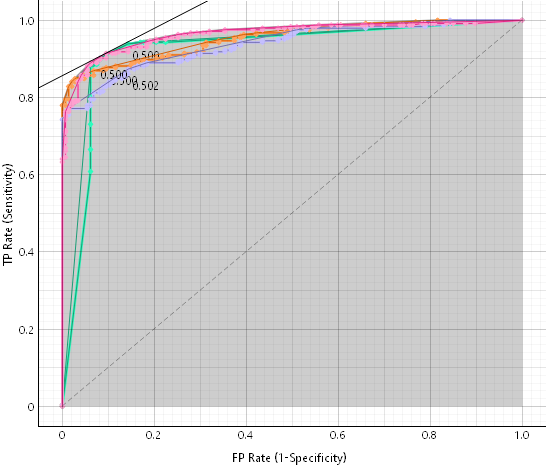
\includegraphics[width=0.4\textwidth]{Resources/ROC_EUA.png}
	\caption{Curva ROC dos Algoritmos - EUA}
\end{figure}

\begin{figure}[!ht]
	\centering
	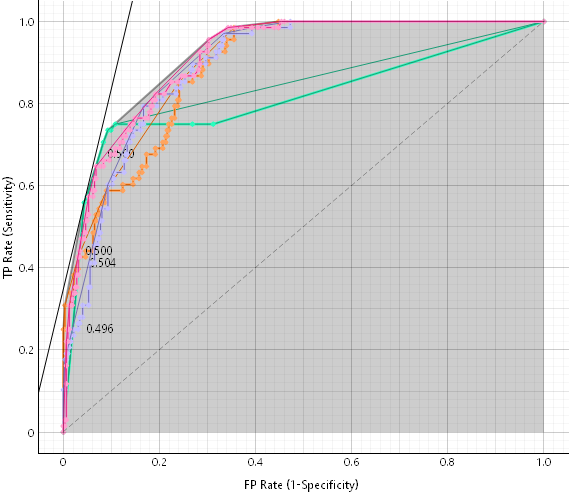
\includegraphics[width=0.4\textwidth]{Resources/ROC_EU.png}
	\caption{Curva ROC dos Algoritmos - Europa}
\end{figure}

\begin{figure}[!ht]
	\centering
	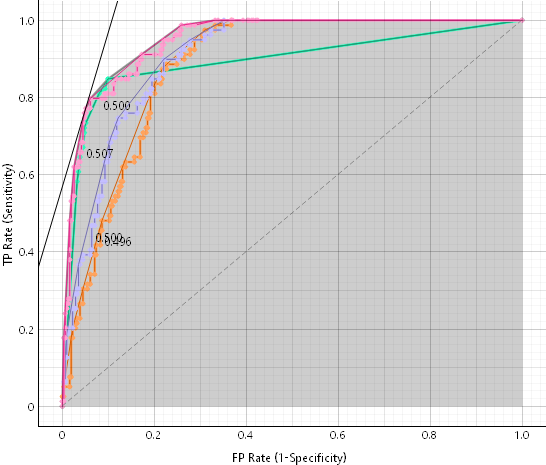
\includegraphics[width=0.4\textwidth]{Resources/ROC_JP.png}
	\caption{Curva ROC dos Algoritmos - Japão}
\end{figure}


%----------------------------------------------------------------------------------------------------------------------------------------------
\newpage
\section{Conclusões}
Concluimos que embora o algoritmo \textit{Tree} seja fácil de interpretar, apresenta limitações em datasets com alta variabilidade,
onde tende a criar divisões muito específicas, resultando em overfitting. Por outro lado, o \textit{Random Forest}, ao agregar várias
árvores, resolve esse problema, mas o custo computacional aumenta significativamente. Já a \textit{Logistic Regression}, apesar da
simplicidade e robustez, pode apresentar dificuldades em modelar relações complexas entre as variáveis. Finalmente, as \textit{Neural Networks}
destacam-se pela capacidade de capturar padrões complexos, mas requerem grandes volumes de dados e longos períodos de treino, podendo
ser menos práticas para problemas pequenos. Em suma, concluimos que a escolha do algoritmo correto é de extrema importância dado que
a precisão, sensibilidade e especificidade deve ser garantida e que a sua eficácia em grande escala tem um grande impacto no resultado final.
No entanto, é importante também destacar algumas limitações do estudo. Primeiramente, o tamanho do dataset, com apenas 400 entradas por coluna,
pode não ser representativo o suficiente para generalizações em larga escala. Além disso, fatores como o viés dos dados
(mais veículos de origem norte-americana) podem ter influenciado os resultados.

\section{Trabalhos Relacionados}
Os trabalhos "Automobile EDA" \cite{ref2} e "EDA CAR INFORMATION DATA" \cite{ref3} são exemplos de trabalhos relacionados com este dataset.
Estes trabalhos tem outras abordagens e análises ao dataset, que tem como objetivo analisar as diferentes caracteristicas dos veículos
em vez de diferentes algoritmos, mesmo assim, são trabalhos foram úteis para uma compreensão mais aprofundada do dataset assim garantindo
um estudo mais rigoroso.

\begin{thebibliography}{1}
	\bibitem{ref1} T. Elmetwally, “Car information dataset”, \textit{Kaggle}, Maio 2023.
	\bibitem{ref2} A. Aboraida, “Automobile EDA”, \textit{Kaggle}, Setembro 2024.
	\bibitem{ref3} V. Salodkar, “EDA CAR INFORMATION DATA”, \textit{Kaggle}, Junho 2023.
\end{thebibliography}

\end{document}
